
\documentclass[12pt,letterpaper]{report}
\usepackage{bbm}
\usepackage{dsfont}
\usepackage{multicol}
\usepackage{lipsum}
\usepackage{mwe}
\usepackage{graphicx}
\usepackage{epstopdf}
\epstopdfsetup{outdir=./}
\usepackage{subcaption}
\usepackage{geometry}
\usepackage{float}
\usepackage{amsmath,amssymb}
\usepackage{makecell}
\usepackage{lmodern}
\usepackage{mathtools}
\usepackage[thinc]{esdiff}
\usepackage{import}
\usepackage{braket}
\usepackage{enumerate}
\usepackage{listings}
\usepackage{biblatex}
\addbibresource{biblio.bib}

\newcommand{\lam}{\lambda}

% Title Page
\title{ Dynamique moléculaire et simulation Monte-Carlo \\ 5: Classical Molecular Dynamics (MD) Simulations}
\author{Bruno Rodriguez Carrillo \\ EPFL}

\geometry{
	a4paper,
	total={185mm,260mm},
	left=15mm,
	top=15mm,
}

\begin{document}	
	\maketitle
	% theory questions
	%### Monte Carlo and Statistical Mechanics
	\section*{MD Initialization and Temperature}
	
	\begin{enumerate}
		\item 
		Implement the initialization described in the Theory section in our ToyMD code in 'toy\_md.py' in the section '\#\#INITIALIZATION HERE\#\#'. For this you should pick random velocities using 'r.random()' which will produce random numbers between '0' and '1'. You need to shift this random gaussian distribution appropriately and then multiply it such that the width of the velocity distribution matches the kinetic energy at the target temperature. Use the variables 'masses[i]' for the mass of particle 'i' and Boltzmann constant '0.0831415'. Remember that for each degree of freedom (e.g velocity in x direction) (5.22) holds.
		
		Since we know that equation (5.22) holds for each degree of freedom, we have for $v^{2}_{x}$:
		
		$$
			E_{kin} = \dfrac{1}{2} k_{B}\cdot T = \dfrac{1}{2} m \cdot v^{2}_{x} \Rightarrow
			v^{2}_{x} = \dfrac{k_{B}\cdot T}{m}
		$$
		
		For $v_{x}$ to follow a normal distribution with zero mean and variance $\sigma^{2} = T$, we have 
		$$
			v_{x} \sim \sqrt{\dfrac{k_{B}\cdot T}{m}} \cdot N(0, 1)
		$$		
		
		We use the same approach for $v_{y}$ and $v_{y}$.
		
		Then a possible implementation is: 
		
		\begin{figure}[H]
			\centering
			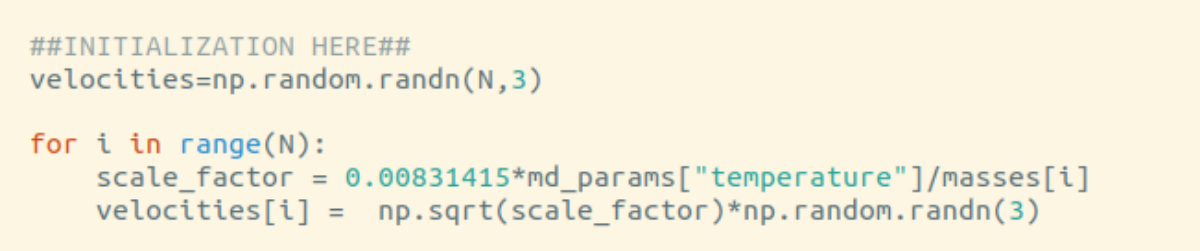
\includegraphics[width=0.7\linewidth]{inititalizationVelo.png}		
			\caption{Velocity re-scale.}
			\label{fig::inititalizationVelo}
		\end{figure}  

		\item
		Implement the Berendsen thermostat in the 'toy\_md.py' and 'toy\_md\_integrate.py' (change the 'compute\_lambda\_T' function) files.
		
		From equation (5.19), we have that:
		
		$$
			\lambda = \sqrt{ 1 + \dfrac{dt}{\tau} \cdot \left( \dfrac{T_{0} }{T} - 1 \right) }
		$$
		
		Then we re-scale each velocity component as $v = \lambda \cdot v$ for each particle too.
		
		As a result, we have the following implementation:
		
		\begin{figure}[H]
			\centering
			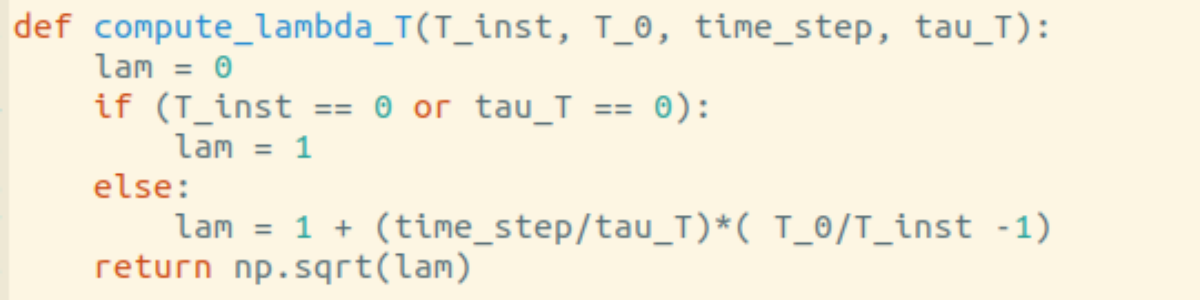
\includegraphics[width=0.6\linewidth]{berendsenLam.png}		
			\caption{Berendsen thermostat lambda computation}
			\label{fig::berendsenLam}
		\end{figure}  
	
		\begin{figure}[H]
			\centering
			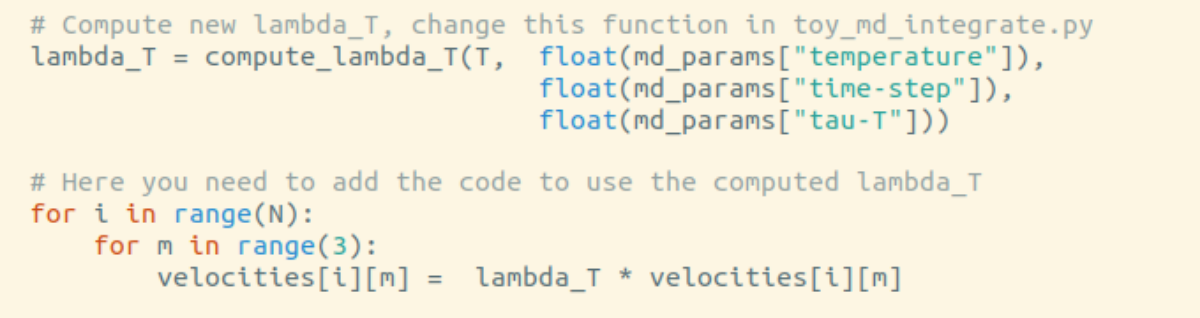
\includegraphics[width=0.6\linewidth]{berendsenVelocity.png}		
			\caption{Berendsen thermostat velocity re-scaling}
			\label{fig::berendsenVelocity}
		\end{figure}  
		
		\item
		A better thermostat is the Andersen thermostat. It can be implemented as follows. Describe what problems this thermostat will present to us e.g for sampling of diffusion coefficients. What advantage does this thermostat have compared to the Berendsen thermostat?
		
		Based on \cite{thijssen_2007}, this method is closest to the experimental situation: the velocity alterations mimic particle collisions with the walls. The rate at which particles should undergo these changes in velocity influences the equilibration time and the kinetic energy fluctuations.	If the rate is high, equilibration will proceed quickly, but as the velocity updates are uncorrelated, they will destroy the long time tail of the velocity autocorrelation function. Moreover, the system will then essentially perform a random walk	through phase space, which means that it moves relatively slowly.
		
		Furthermore, the Nosé and the Andersen methods yield precise canonical distributions for position and momentum coordinates. However, for the Andersen method, it is not always clear at which rate the velocities are to be altered.
		
		On the other hand, Berendsen thermostat does not reproduce the canonical distribution.
		
	\end{enumerate}
  
  \section*{Sampling Configurational Space}
  Open the resulting trajectory in VMD and plot the bond distance of a $C-O$ bond. What to you observe?
  
  \begin{enumerate}
  	\item 
	Plot the distribution of the $CO$ and $OO$ bond lengths during the simulation. How do the sampled values correspond to the values set in the force field?
	
	\begin{figure}[H]
		\centering
		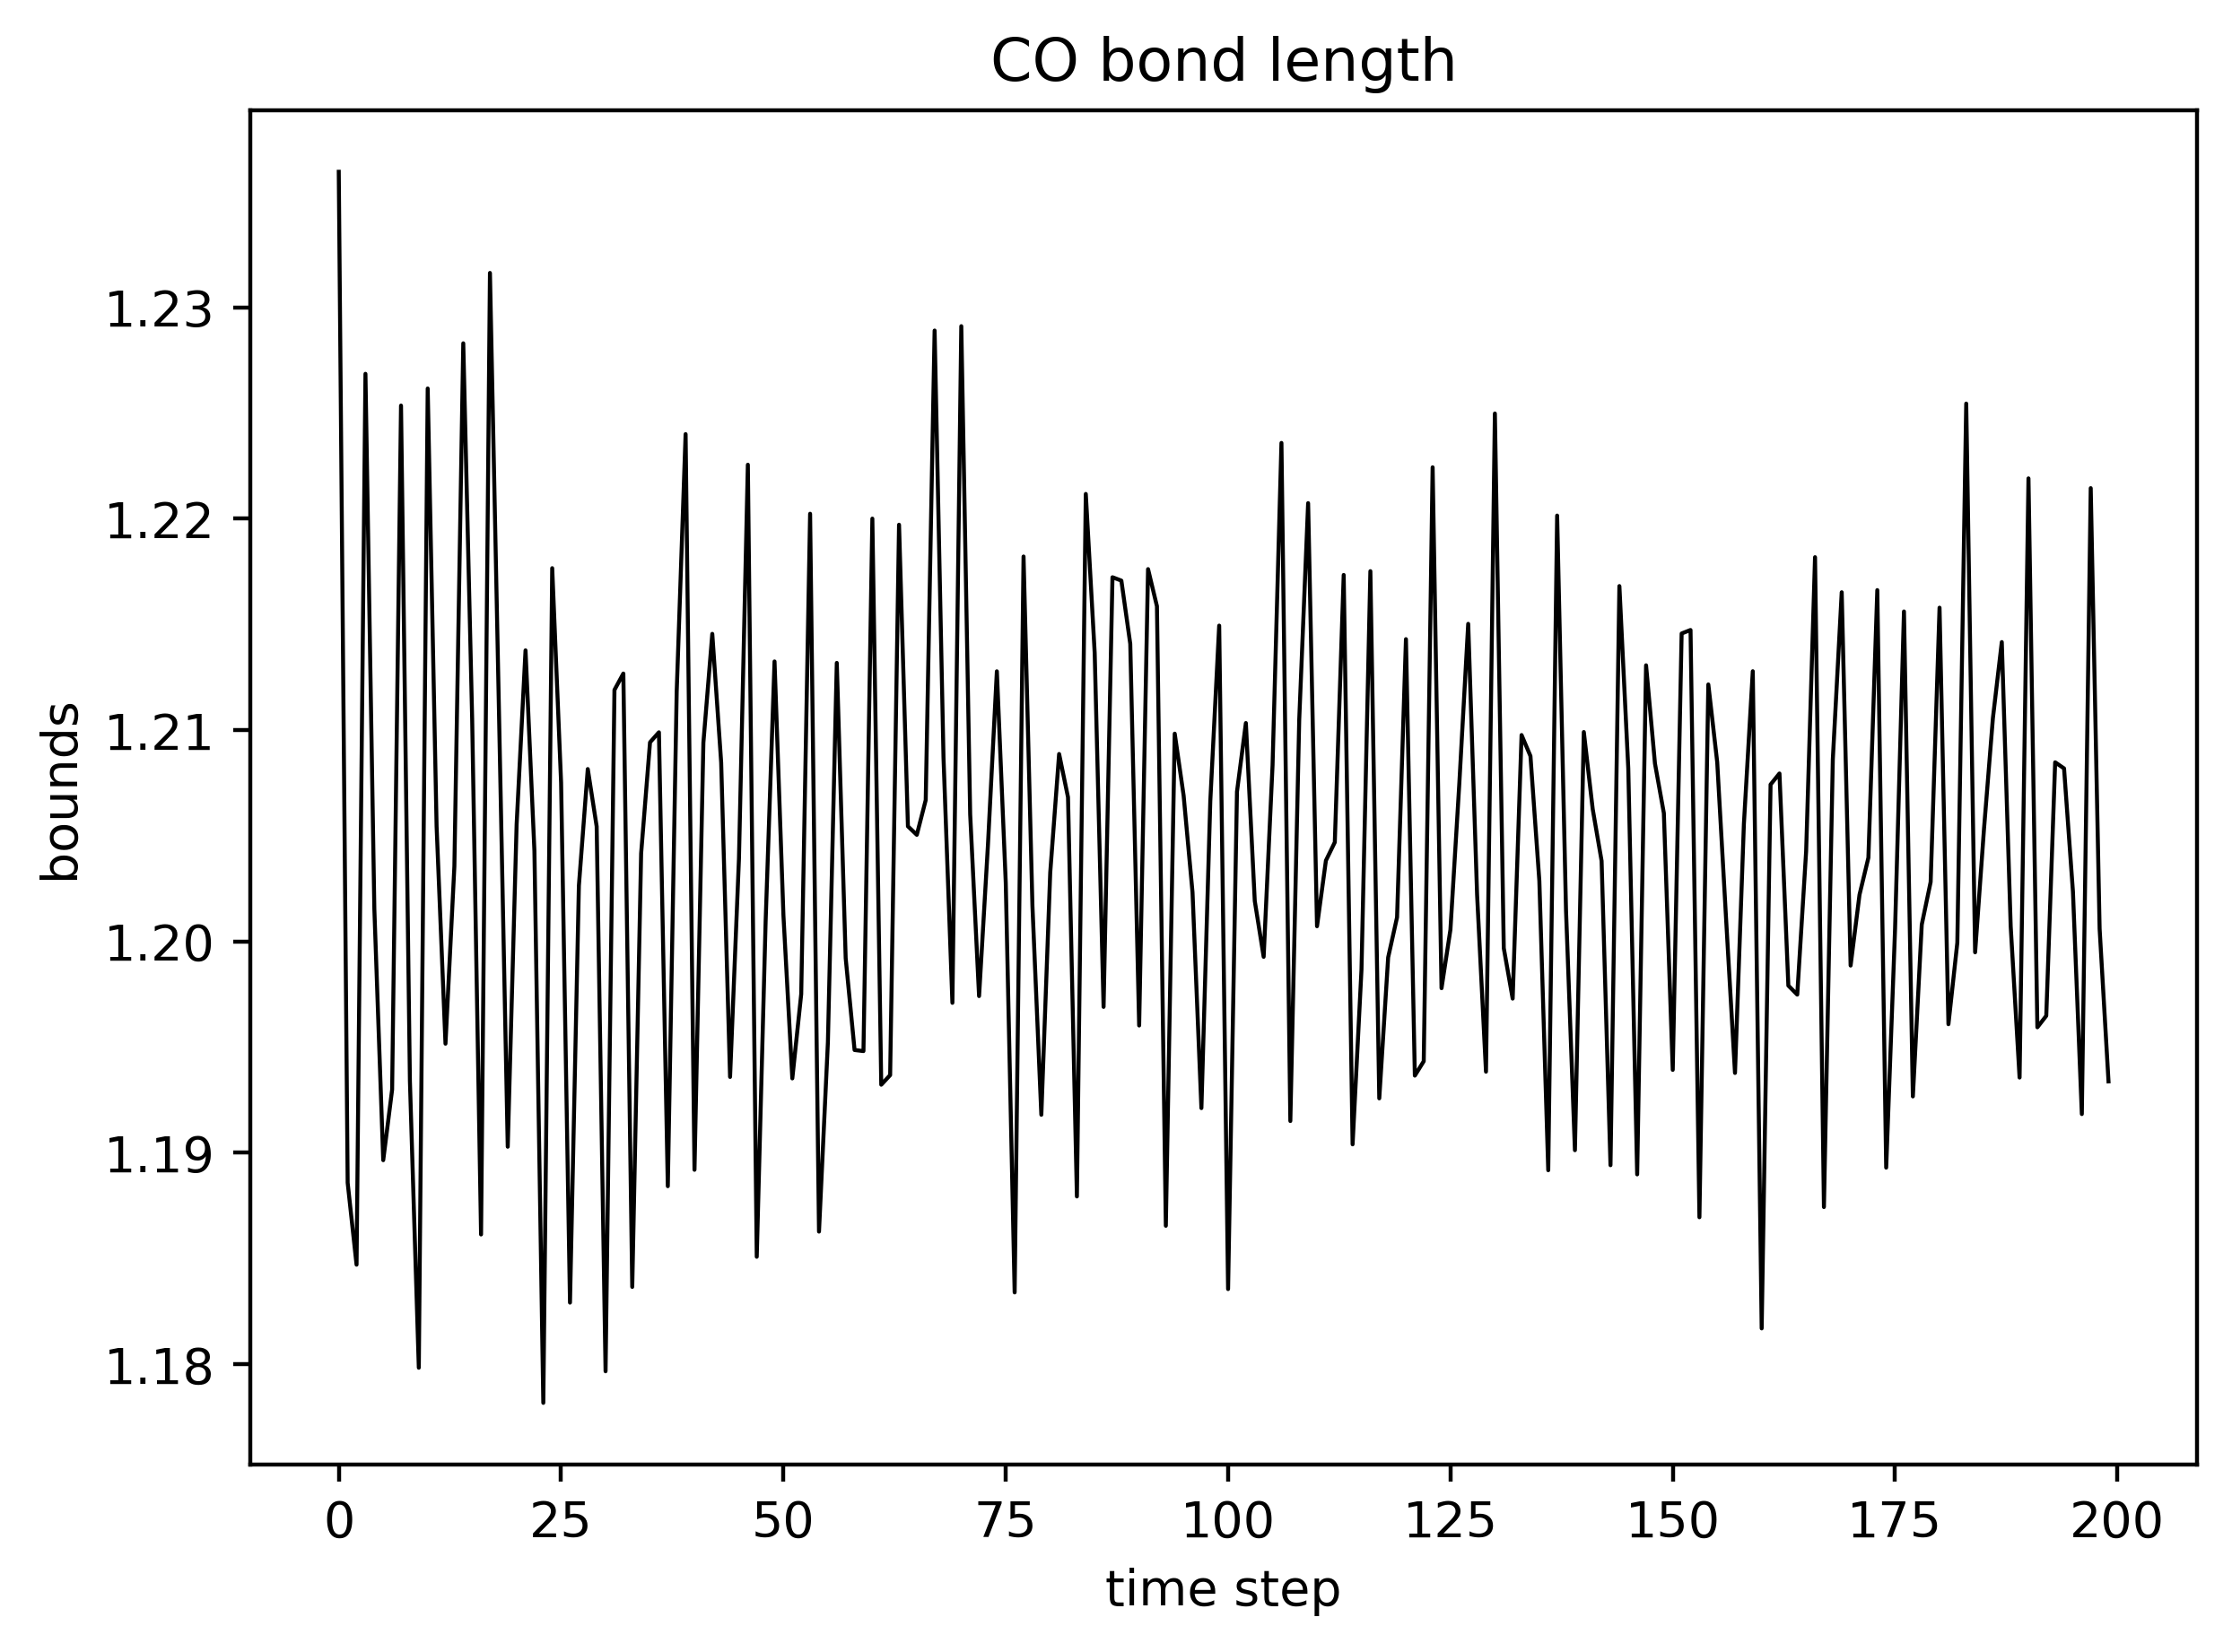
\includegraphics[width=0.6\linewidth]{co.png}		
		\caption{CO bond length.}
		\label{fig::co_bound}
	\end{figure}  

	\begin{figure}[H]
		\centering
		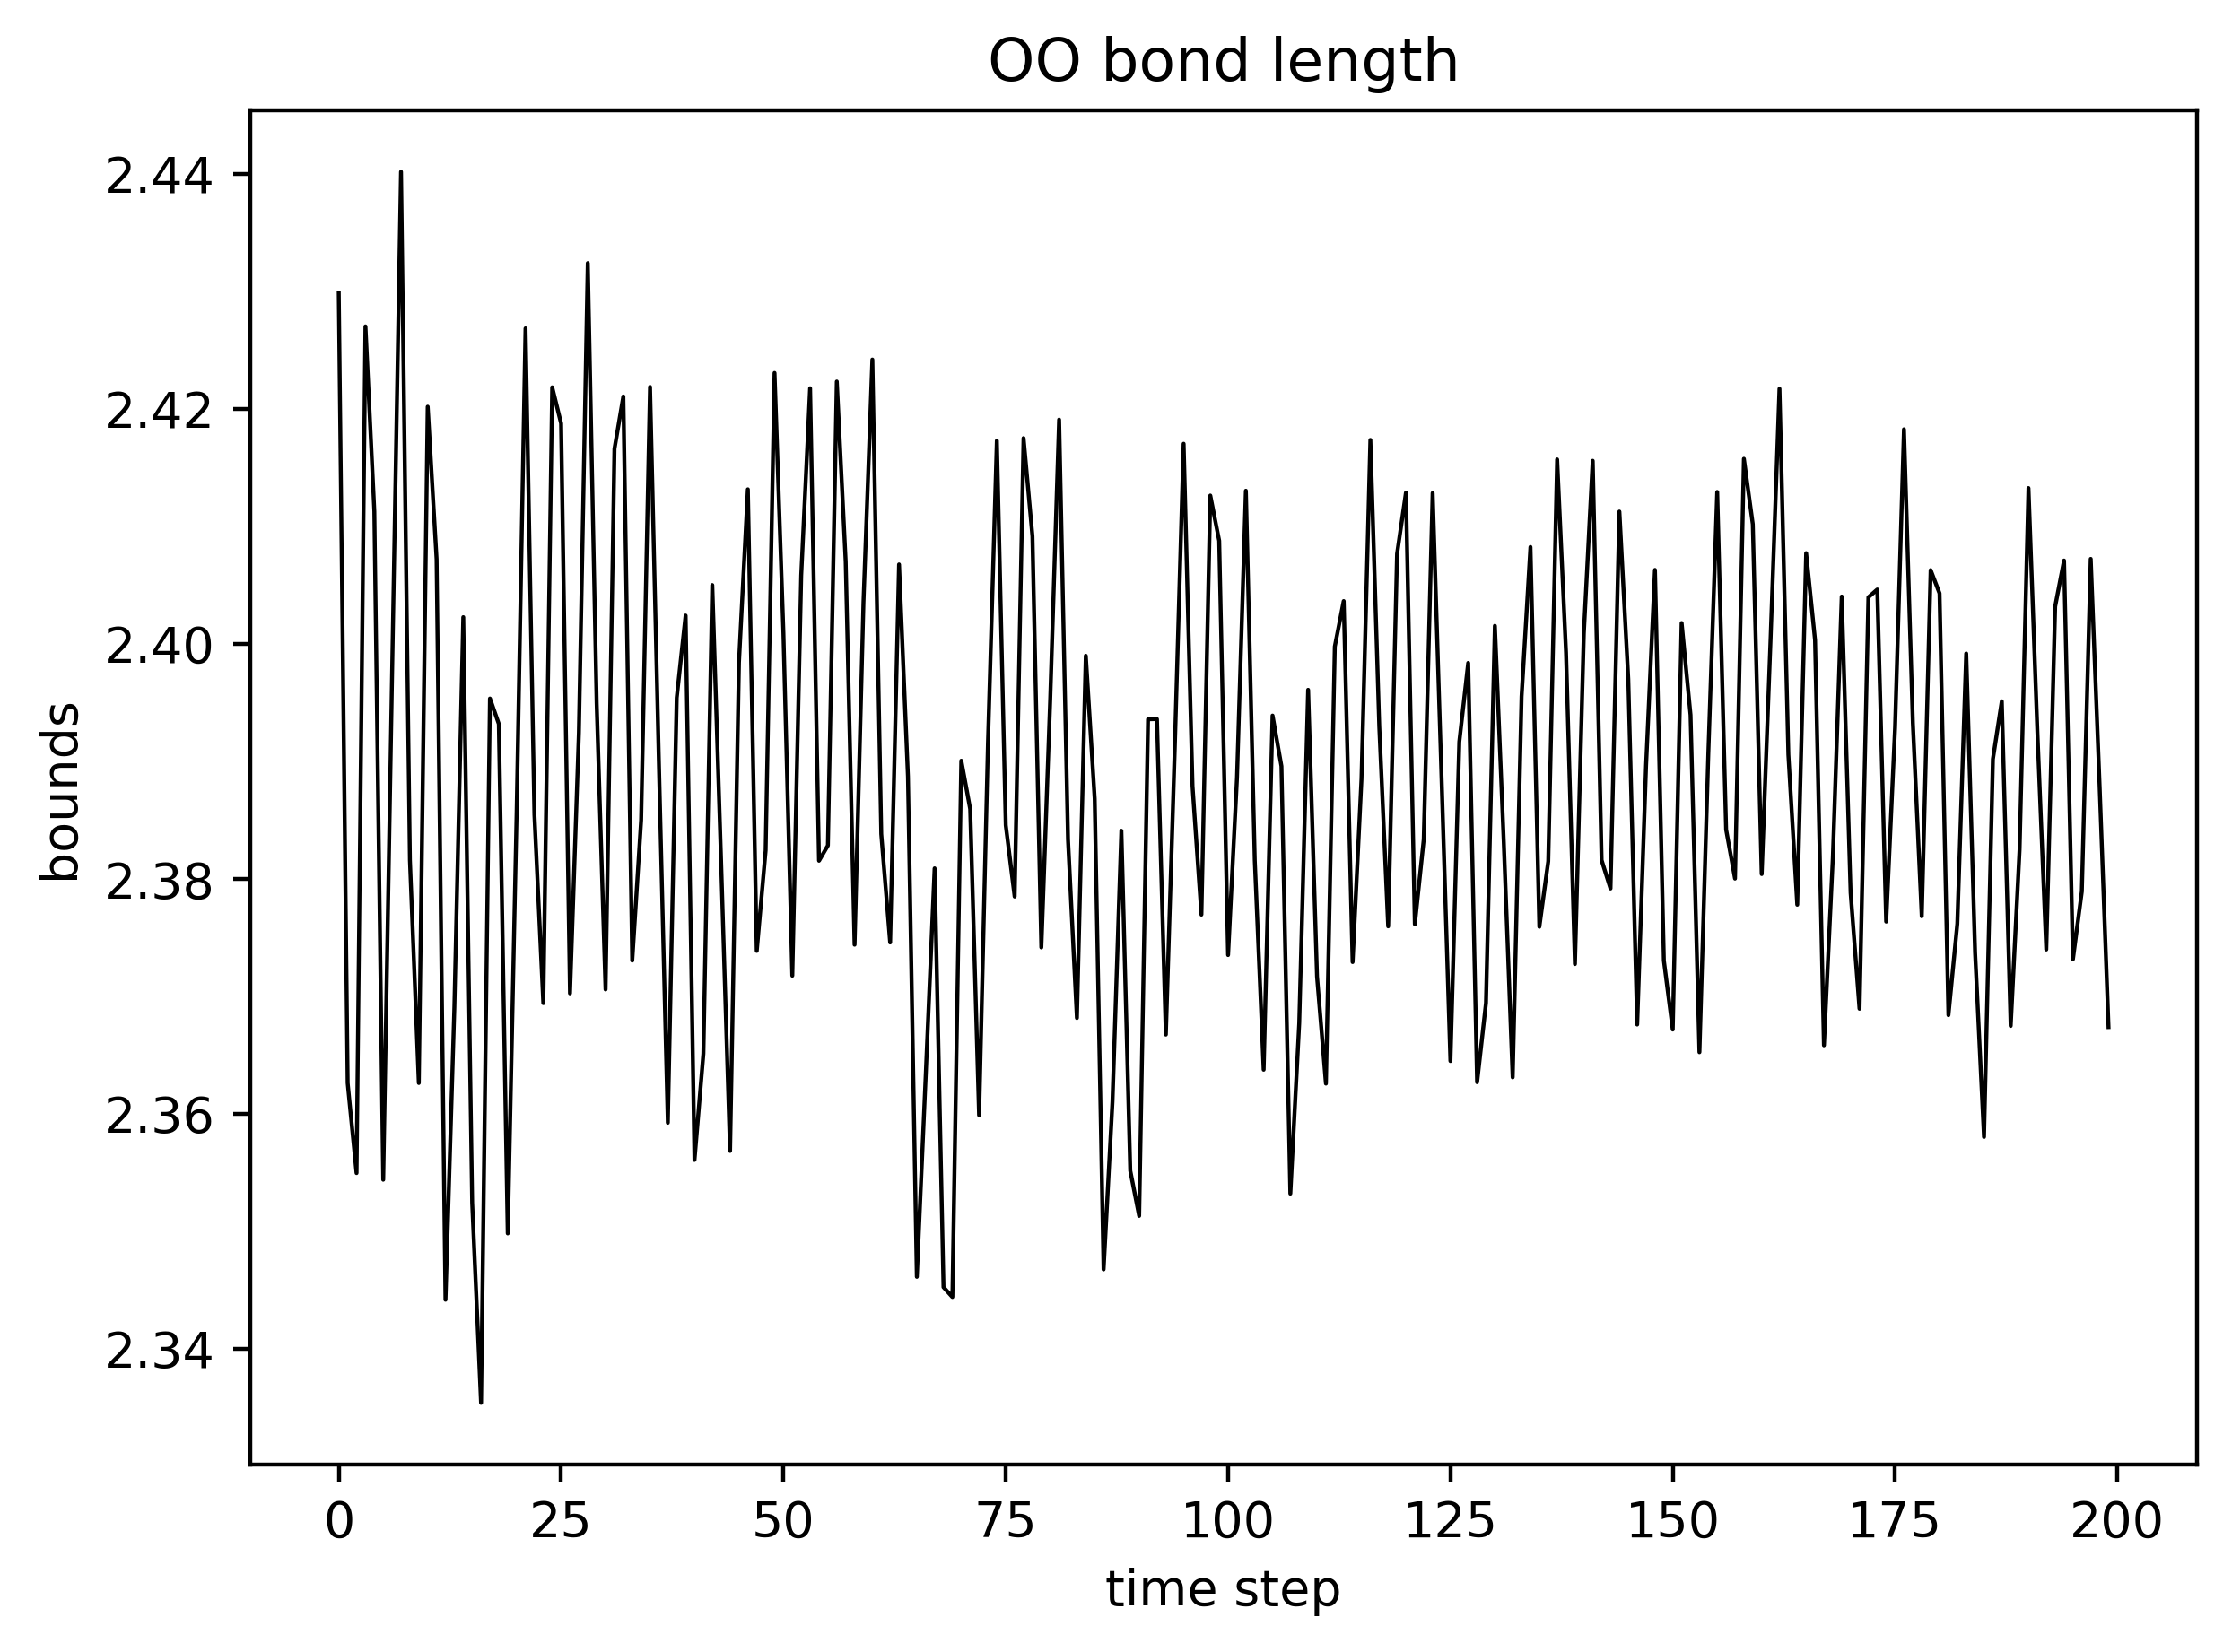
\includegraphics[width=0.6\linewidth]{oo.png}		
		\caption{OO bond length.}
		\label{fig::oo_bound}
	\end{figure}
	
	From \cite{pang_2006}, we should bear in mind that sometimes we have to deal with large molecular systems, such as biopolymers. In these cases, the bond length of a pair of nearest neighbors does not change very much even though the angle between a pair of nearest bonds does.
	If we want to obtain accurate simulation results, we have to choose a time step	much smaller than the period of the vibration of each pair of atoms. This costs	a lot of computing time and might exclude the applicability of the simulation to more complicated systems, such as biopolymers.
	
	The observed lengths correspond to the first term in equation (5.15). Such a force tries to keep the atoms of a fixed molecule together. This also means that the repulsion and attraction forces acting are such that the length of the bonds is kept constant throughout the simulation time. This is the reason why we observe an oscillating behavior around a value. If the length changed abruptly, it would probably mean that the molecule is destroyed because of other forces like the one generated by the Leonard Jones potential acting on molecules. 
	
  	\item 
  	Visualize the radial distribution function of the $CO_2$ trajectory. What do you observe? Bonus: What would you observe for a heterogenous system (i.e a polar molecule solvated in liquid $CO_2$)?

	\begin{figure}[H]
	\centering
	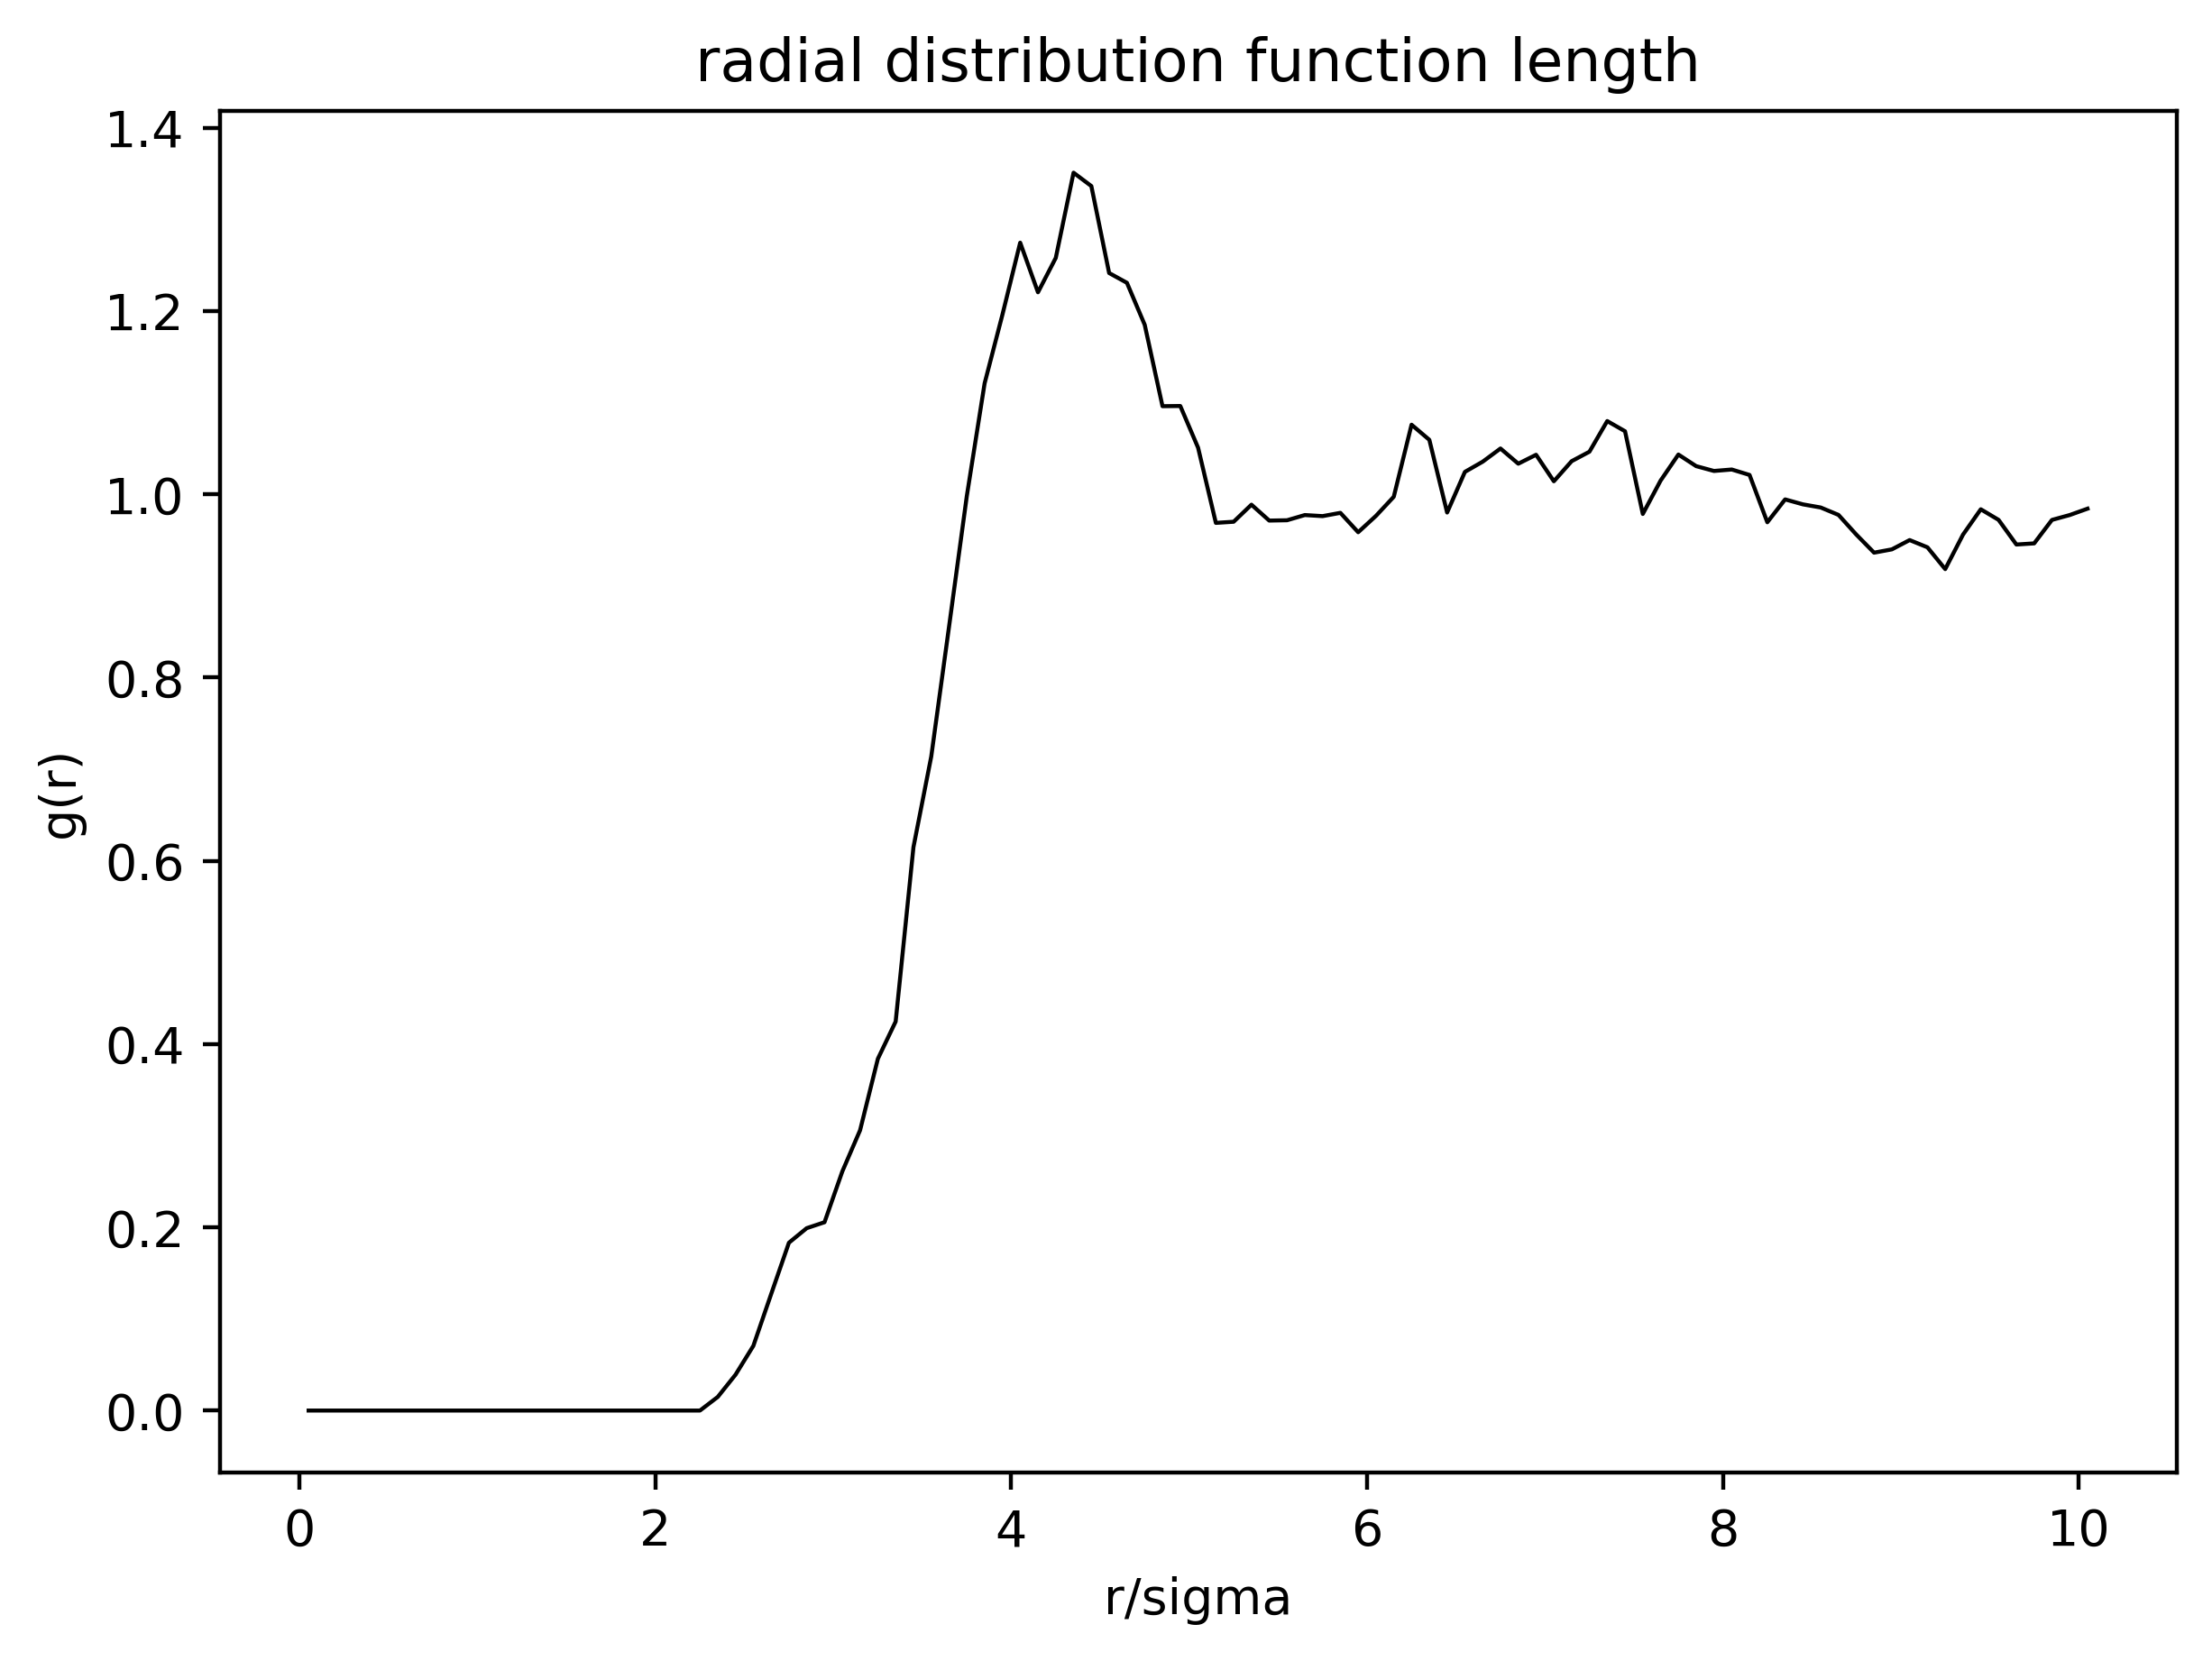
\includegraphics[width=0.5\linewidth]{radial.png}		
	\caption{Radial distribution function of the $CO_2$ trajectory.}
	\label{fig::radial}
	\end{figure}	
		
	From \cite{thijssen_2007}, we have that the pair correlation function contains information concerning the local structure of a fluid. Suppose we were to sit somewhere in the fluid and watch the surroundings for some time, then, on average, we would see a homogeneous structure. Now, If we move along with a particular particle, however, and watch the scenery from this particle's perspective, we will find no particles close to us because of the strong short-range repulsion. Then we have an increase in density due to a layer of particles surrounding our particle, followed by a drop in density marking the boundary between this layer and a second layer, and so on. Because of the fluctuations, the layer structure becomes more and more diffuse for increasing distances and the correlation function will approach a constant value at large distances, as we observe in the plot above. 

  \end{enumerate}
	
	\section*{Timestep and coupling}
	\begin{enumerate}
		\item
		Test the influence of the coupling parameter $\tau$ and timestep $dt$. You set both of those parameters in params.txt. Test 3 different settings of $\tau$ and $dt$ and describe what you observe. 
		
		When $\tau$ tends to infinity, we observe that the Berendsen thermostat is inactive since we have $\dfrac{dT}{dt} = 0$ and then we are just implementing velocity re-scaling by a factor of 1 ($\lambda = 1$); hence, temperature fluctuations are allowed. The reason why this happens is that the velocities are first generated according to the re-scaling $v_{x} \sim \sqrt{\dfrac{k_{B}\cdot T}{m}} \cdot N(0, 1)$. Thus temperature fluctuations will vary until they reach the appropriate value of a microcanonical ensemble.	Even thought temperature fluctuates, we are not sampling the NVT ensemble but the isokinetic one. This is the case when $\tau > > dt$.
		
		On the other hand, too small values of $\tau$ will cause abrupt temperature fluctuations, in this case $dt > > \tau$.
		When $\tau = dt$, the Berendsen thermostat is a velocity scaling from one time step to another. As a result, the dynamics generated in this case is not realistic. 
		
		We should also point out that the $dt$ parameter is the one used during the Verlet algorithm and such a number determines in some sense the accuracy of our values. As it is well known, too small values of $dt$ will generate more precise results but at the same time computational cost will grow. 
		
	\end{enumerate}
	
	\newpage
	\printbibliography

\end{document}    